\documentclass[11pt]{article}

\usepackage[a4paper,margin=0.92in]{geometry}
\usepackage[T1]{fontenc}
\usepackage[utf8]{inputenc}
\usepackage{lmodern}
\usepackage{microtype}
\usepackage{amsmath,amssymb,amsthm,mathtools}
\usepackage{booktabs,array}
\usepackage{graphicx}
\usepackage{enumitem}
\usepackage{xcolor}
\usepackage[hidelinks]{hyperref}

\graphicspath{{../figures/}}

\hypersetup{
  pdftitle={Pandrosion Prime Atlases and the Riemann Critical Line},
  pdfauthor={Ivan Besevic},
  pdfsubject={Pandrosion geometry, Euler factors, Riemann zeta, critical line},
  pdfkeywords={Pandrosion, Riemann zeta, Euler product, critical line, Thales scaling, Riemann inversion}
}

\newtheorem{definition}{Definition}[section]
\newtheorem{proposition}[definition]{Proposition}
\newtheorem{theorem}[definition]{Theorem}
\newtheorem{conjecture}[definition]{Conjecture}
\newtheorem{remark}[definition]{Remark}

\newcommand{\C}{\mathbb C}
\newcommand{\R}{\mathbb R}
\newcommand{\N}{\mathbb N}
\newcommand{\Pset}{\mathcal P}
\newcommand{\E}{\mathcal E}
\newcommand{\A}{\mathcal A}
\newcommand{\Z}{\mathcal Z}
\newcommand{\eps}{\varepsilon}
\newcommand{\dd}{\,\mathrm d}
\DeclareMathOperator{\Ree}{Re}
\DeclareMathOperator{\Imm}{Im}

\title{Pandrosion Prime Atlases and the Riemann Critical Line\\[3pt]
\large Euler factors as infinite geometric charts}
\author{Ivan Besevic\\Independent Mathematical Research}
\date{May 2026}

\begin{document}
\maketitle

\begin{abstract}
This paper proposes a new way to connect the geometric Pandrosion method of
Paper 000 with the Riemann zeta function.  The connection is not the finite
identity
\(\sum_k 1/P'(\lambda_k)=0\), which is classical Lagrange interpolation.  The
connection is instead the logarithmic chart geometry behind the Euler product.
Paper 000 shows that the monomial map for \(z^p=x\) is governed by the finite
geometric sum
\[
        S_p(s)=1+s+\cdots+s^{p-1},
\]
and that the correct geometry first chooses a Thales homothety and, when
needed, a reciprocal Riemann chart so that a normalized target lies close to
\(1\).  For the zeta function, every Euler factor is an infinite geometric
Pandrosion cell:
\[
        \frac{1}{1-\ell^{-s}}
        =1+\ell^{-s}+\ell^{-2s}+\cdots.
\]
We therefore define a prime-by-prime Pandrosion atlas with direct chart
\(q_\ell(s)=\ell^{-s}\) and reciprocal chart
\(q_\ell^\infty(s)=\ell^{-(1-s)}\).  The involution \(s\mapsto1-s\), which is
the symmetry axis of the completed zeta functional equation, becomes the
global version of the Riemann-chart inversion from Paper 000.

The main rigorous observation is finite and geometric.  For any finite set of
primes and any positive weights, the logarithmic direct and reciprocal chart
costs
\[
        \E_+(\sigma)=\sum_{\ell}w_\ell(\sigma\log\ell)^2,\qquad
        \E_\infty(\sigma)=\sum_{\ell}w_\ell((1-\sigma)\log\ell)^2
\]
are balanced at exactly \(\sigma=1/2\).  Thus the critical line is the unique
Thales--Riemann equilibrium line of the prime Pandrosion atlas.  This is not a
proof of the Riemann hypothesis.  It is a new geometric formulation: the
critical line is where the direct Euler charts and reciprocal Euler charts have
equal logarithmic distortion, and the nontrivial zeros may be viewed as phase
destruction events on that balanced atlas.
\end{abstract}

\paragraph{One-sentence summary.}
Euler factors are infinite Pandrosion geometric sums, and the critical line
\(\Re(s)=1/2\) is the chart-equilibrium locus between the direct prime chart
\(\ell^{-s}\) and the reciprocal prime chart \(\ell^{-(1-s)}\).

\paragraph{Status.}
The atlas construction and critical-line balance theorem are elementary and
proved below.  The proposed interpretation of zeta zeros as balanced-atlas
phase destruction is a research program, not a proof of the Riemann hypothesis.

\tableofcontents

\section{Motivation}

The legacy Riemann note used Pandrosion language for random matrices, zeta
zeros, and polynomial spectral identities.  Some of its formulas are useful as
notation, but many of the algebraic identities are classical.  For example,
if \(P(z)=\prod_k(z-\lambda_k)\) has simple roots, then
\[
        P'(\lambda_k)=\prod_{j\ne k}(\lambda_k-\lambda_j),
        \qquad
        \sum_k\frac{1}{P'(\lambda_k)}=0
\]
for degree at least \(2\).  This is not a new route to the zeta function.

The more distinctive Pandrosion structure in Paper 000 is different.  It is
the combination of:
\begin{enumerate}[leftmargin=2em]
\item finite geometric sums \(S_p\);
\item logarithmic normalization by homothety;
\item reciprocal Riemann-chart inversion;
\item choosing the chart that keeps \(|\log y|\) small.
\end{enumerate}
The Riemann zeta function is naturally built from logarithmic scales:
\[
        \zeta(s)=\prod_{\ell\ {\rm prime}}\frac{1}{1-\ell^{-s}}.
\]
This suggests using the Euler product itself as the bridge from Pandrosion
geometry to zeta.

\section{From monomial Pandrosion to Euler cells}

In Paper 000 the basic monomial denominator is
\[
        S_p(s)=1+s+\cdots+s^{p-1}.
\]
For a prime \(\ell\) and a complex variable \(s\), put
\[
        q_\ell(s)=\ell^{-s}.
\]
The finite Euler-Pandrosion cell of depth \(N\) is
\[
        E_{\ell,N}(s)
        =S_N(q_\ell(s))
        =1+\ell^{-s}+\ell^{-2s}+\cdots+\ell^{-(N-1)s}.
\]
For \(\Re(s)>0\), \(E_{\ell,N}(s)\) converges as \(N\to\infty\) to the Euler
factor:
\[
        E_{\ell,\infty}(s)=\frac{1}{1-\ell^{-s}}.
\]

\begin{definition}[Euler-Pandrosion product]
For a finite prime set \(\Pset\) and depth \(N\), define
\[
        \Z_{\Pset,N}(s)
        =
        \prod_{\ell\in\Pset}E_{\ell,N}(s).
\]
When \(N=\infty\) and \(\Pset\) increases over all primes, this tends to
\(\zeta(s)\) in the half-plane \(\Re(s)>1\).
\end{definition}

Thus zeta is not merely analogous to Pandrosion.  In the Euler half-plane it is
a limiting product of infinite Pandrosion geometric cells.

\begin{figure}[htbp]
\centering
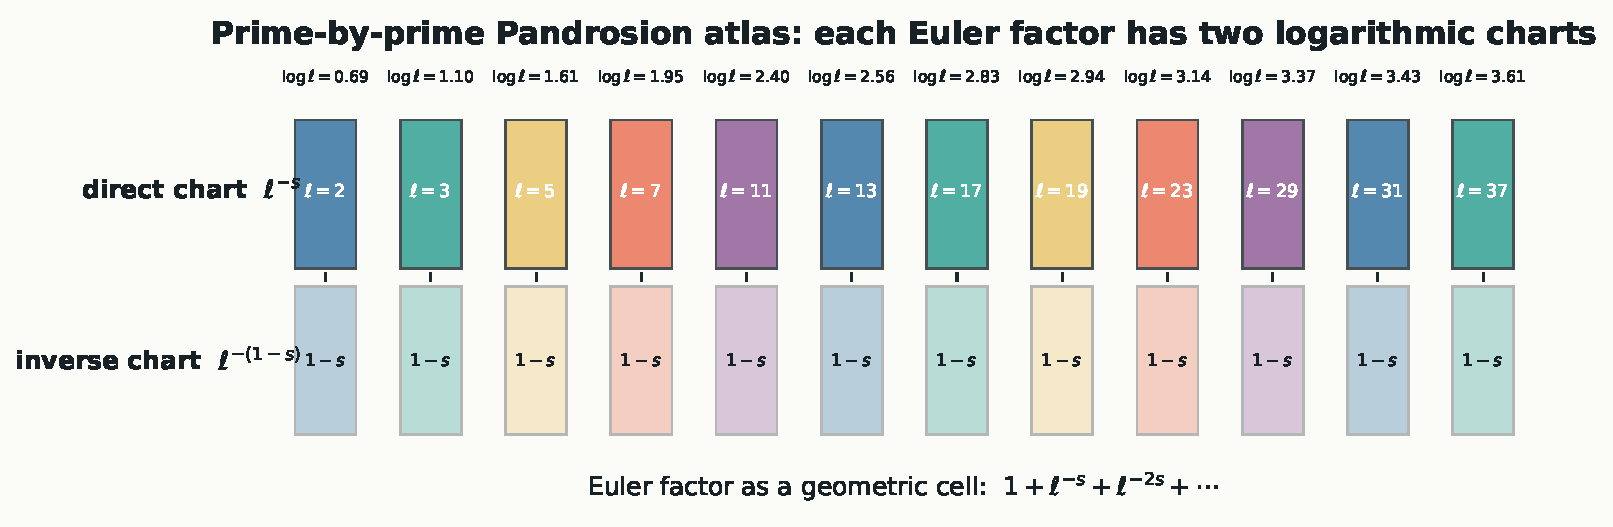
\includegraphics[width=0.98\linewidth]{025_prime_atlas_cells.pdf}
\caption{Prime-by-prime Pandrosion atlas.  Each prime contributes a direct
Euler cell \(1+\ell^{-s}+\ell^{-2s}+\cdots\) and a reciprocal cell obtained by
the involution \(s\mapsto1-s\).}
\label{fig:prime-atlas}
\end{figure}

\section{The reciprocal chart and the functional-equation axis}

The reciprocal Riemann chart in Paper 000 moves a small or badly scaled target
into a normalized chart before iteration.  For Euler factors the analogous
operation is the involution
\[
        s\longmapsto1-s.
\]
It sends the direct prime coordinate \(q_\ell(s)=\ell^{-s}\) to the reciprocal
prime coordinate
\[
        q_\ell^\infty(s)=\ell^{-(1-s)}.
\]
This is not yet the full zeta functional equation; the completed zeta function
\[
        \xi(s)=\frac12 s(s-1)\pi^{-s/2}\Gamma(s/2)\zeta(s)
\]
also contains the gamma and conductor terms.  The point is geometric: the same
involution that underlies the completed functional equation is the global
prime-atlas version of the Riemann-chart inversion in the monomial paper.

\begin{definition}[Prime-atlas chart costs]
Let \(\Pset\) be a finite set of primes and \(w_\ell>0\).  For
\(\sigma=\Re(s)\), define
\[
        \E_+(\sigma)
        =
        \sum_{\ell\in\Pset}w_\ell(\sigma\log\ell)^2,
        \qquad
        \E_\infty(\sigma)
        =
        \sum_{\ell\in\Pset}w_\ell((1-\sigma)\log\ell)^2.
\]
The selected atlas cost is
\[
        \E_{\rm sel}(\sigma)=\min(\E_+(\sigma),\E_\infty(\sigma)).
\]
\end{definition}

The squared logarithmic costs are the direct analogues of the
\(|\log y|\)-based chart rule in Paper 000.  The direct chart measures how far
\(\ell^{-s}\) is from unit scale; the inverse chart measures the same quantity
after \(s\mapsto1-s\).

\begin{theorem}[Critical line as Pandrosion chart equilibrium]
For every finite nonempty prime set \(\Pset\) and every positive weight family
\((w_\ell)\), the equality
\[
        \E_+(\sigma)=\E_\infty(\sigma)
\]
holds if and only if \(\sigma=1/2\).  Equivalently, the line
\(\Re(s)=1/2\) is the unique direct/reciprocal chart-equilibrium locus of the
prime Pandrosion atlas.
\end{theorem}

\begin{proof}
Subtract the two costs:
\[
        \E_+(\sigma)-\E_\infty(\sigma)
        =
        \sum_{\ell\in\Pset}w_\ell
        \left(\sigma^2-(1-\sigma)^2\right)(\log\ell)^2.
\]
Since
\[
        \sigma^2-(1-\sigma)^2=2\sigma-1,
\]
we get
\[
        \E_+(\sigma)-\E_\infty(\sigma)
        =
        (2\sigma-1)
        \sum_{\ell\in\Pset}w_\ell(\log\ell)^2.
\]
The sum is strictly positive.  Hence equality is equivalent to
\(2\sigma-1=0\), i.e. \(\sigma=1/2\).
\end{proof}

\begin{figure}[htbp]
\centering
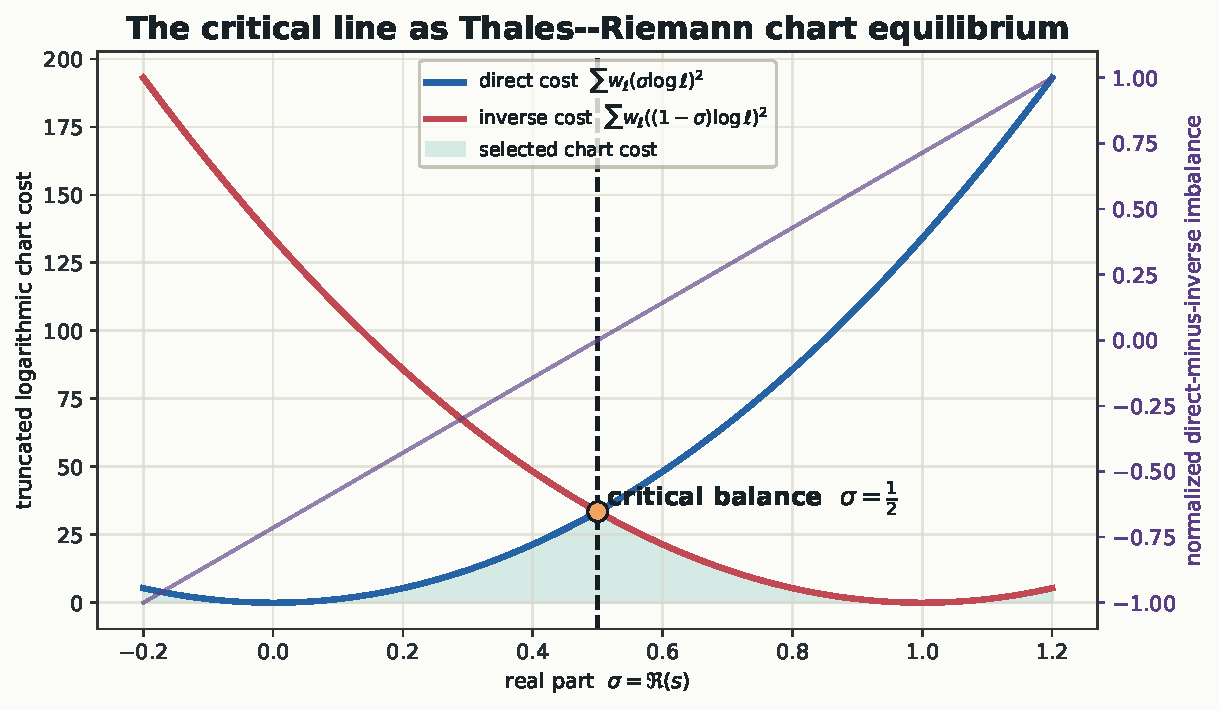
\includegraphics[width=0.86\linewidth]{025_critical_line_balance.pdf}
\caption{The critical line as chart equilibrium.  Direct and reciprocal
logarithmic distortions are equal exactly at \(\sigma=1/2\), independently of
the positive weights assigned to the finite prime atlas.}
\label{fig:critical-balance}
\end{figure}

\section{Phase, cancellation, and zeros}

The balance theorem explains why the critical line is geometrically special,
but it does not locate zeros.  Zeros require phase cancellation.  Write
\[
        q_\ell(\sigma+it)=\ell^{-\sigma}e^{-it\log\ell}.
\]
The modulus is controlled by the chart coordinate \(\sigma\); the phase rotates
with frequency \(\log\ell\).  The primes therefore generate an incommensurate
family of rotating geometric cells.

\begin{definition}[Balanced Euler-Pandrosion phase field]
For a finite prime set and finite depth, define
\[
        \Phi_{\Pset,N}(s)
        =
        \arg \prod_{\ell\in\Pset}E_{\ell,N}(s),
\]
away from zeros of the truncated product.  On the critical line this becomes
\[
        \Phi_{\Pset,N}(1/2+it).
\]
\end{definition}

In this language, a zero of a completed limiting object is not a mysterious
point attached to a finite interpolation identity.  It is a destructive phase
event in an infinite balanced geometric atlas.

\begin{conjecture}[Pandrosion prime-atlas cancellation principle]
After the gamma/conductor normalization required by the completed zeta
function, nontrivial zeta zeros are limiting phase-destruction events of the
balanced prime Pandrosion atlas.  The line \(\Re(s)=1/2\) is selected not by a
finite polynomial vanishing identity, but by the equality of direct and
reciprocal logarithmic chart distortions prime by prime.
\end{conjecture}

\begin{figure}[htbp]
\centering
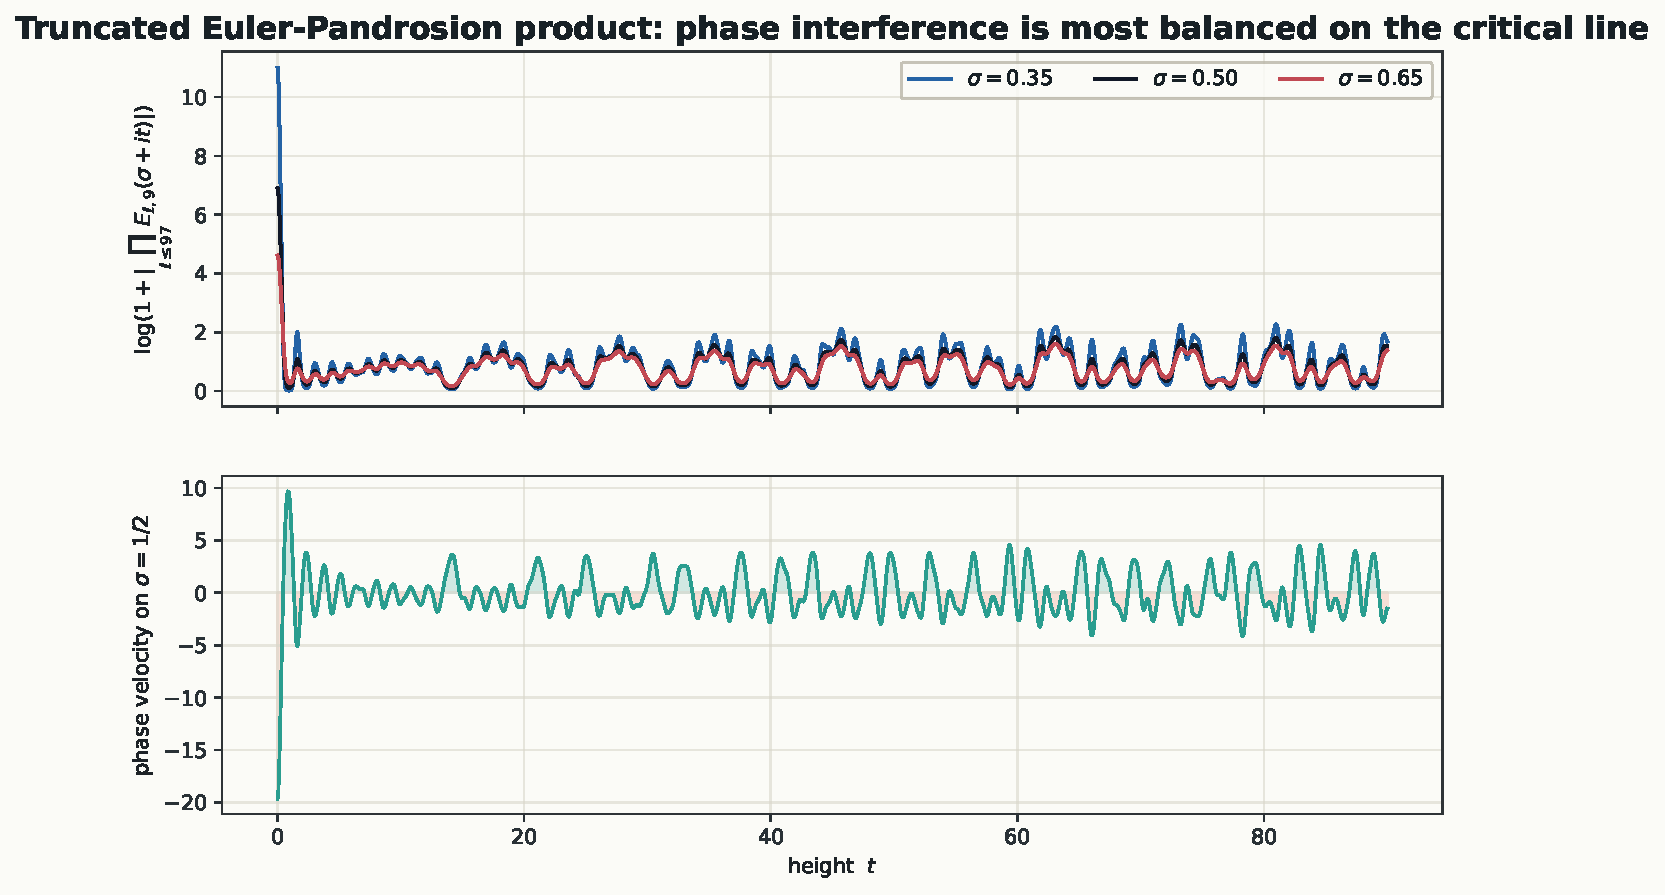
\includegraphics[width=0.96\linewidth]{025_euler_pandrosion_interference.pdf}
\caption{A finite numerical illustration, not evidence for the Riemann
hypothesis.  The product \(\prod_{\ell\le97}E_{\ell,9}(\sigma+it)\) shows
phase interference from the prime logarithms.  The critical-line trace is the
balanced direct/reciprocal chart slice.}
\label{fig:interference}
\end{figure}

\section{Relation to the completed zeta function}

The Euler product alone converges only in \(\Re(s)>1\).  Any serious relation
to the critical strip must include the completed function
\[
        \xi(s)=\frac12s(s-1)\pi^{-s/2}\Gamma(s/2)\zeta(s),
        \qquad
        \xi(s)=\xi(1-s).
\]
In the present framework the gamma/conductor factor should be treated as the
archimedean chart, while the Euler factors are the non-archimedean prime
charts.  Thus the full object is not a single prime product; it is an
adelic-style Pandrosion atlas:
\[
        \text{archimedean chart}
        \quad+\quad
        \text{prime geometric charts}.
\]
The finite theorem above explains the prime-side equilibrium.  The completed
functional equation says that the archimedean chart respects the same
involution.

\section{What is new and what is not}

The following distinctions are important.

\begin{enumerate}[leftmargin=2em]
\item The identity
\(\sum_k1/P'(\lambda_k)=0\) is classical and should not be advertised as a new
formula.
\item Euler products and the functional equation of \(\zeta\) are classical.
\item The new proposal is the geometric reading: Euler factors are infinite
Pandrosion sums, \(s\mapsto1-s\) is the global Riemann-chart inversion, and
\(\Re(s)=1/2\) is the unique logarithmic chart-equilibrium line of the prime
atlas.
\item The zero interpretation is conjectural.  It reframes the problem in
terms of balanced-atlas phase cancellation; it does not prove that all zeros
lie on the critical line.
\end{enumerate}

\section{Research program}

This viewpoint suggests concrete next steps.

\begin{enumerate}[leftmargin=2em]
\item Add the archimedean gamma chart explicitly and define a completed
Pandrosion atlas whose involution is exactly \(s\mapsto1-s\).
\item Replace the elementary quadratic chart cost by a natural energy derived
from \(\log|\xi(s)|\) or from the argument principle.
\item Study whether off-critical points have unavoidable direct/reciprocal
chart imbalance after completion.
\item Compare the phase velocity of truncated Euler-Pandrosion products with
known zero-counting formulas and the Riemann--Siegel theta term.
\item Revisit CUE/GUE statistics only after the prime-atlas construction is in
place, so random matrices model balanced-atlas phase statistics rather than
replace the Pandrosion geometry.
\end{enumerate}

\section{Conclusion}

The cleanest link between Paper 000 and the Riemann zeta function is not the
finite spectral identity of the legacy Riemann note.  It is the fact that every
Euler factor is an infinite geometric Pandrosion cell and that the zeta
functional equation uses the same direct/reciprocal involution as the
Riemann-chart logic of monomial Pandrosion.  In this prime-atlas geometry, the
critical line is not inserted by hand: it is the unique locus where direct and
reciprocal logarithmic chart costs are equal.  This gives a genuinely geometric
Pandrosion formulation of the critical line, and a precise research program for
turning phase-cancellation heuristics into testable mathematics.

\begin{thebibliography}{99}

\bibitem{Besevic000}
I. Besevic, \emph{A Monomial Pandrosion Scheme: Contraction, Chart Scaling,
and Steffensen Acceleration for \(z^p=x\)}, preprint, May 2026.

\bibitem{Besevic001}
I. Besevic, \emph{Chart-Scaled Cubic Pandrosion by Finite-Slope Halley
Acceleration}, preprint, May 2026.

\bibitem{Besevic009}
I. Besevic, \emph{Pandrosion Atlases and Dynamic Geometric Charts}, preprint,
May 2026.

\bibitem{Riemann}
B. Riemann, ``Ueber die Anzahl der Primzahlen unter einer gegebenen
Grosse,'' \emph{Monatsberichte der Berliner Akademie}, 1859.

\bibitem{Titchmarsh}
E. C. Titchmarsh, \emph{The Theory of the Riemann Zeta-Function}, 2nd ed.,
revised by D. R. Heath-Brown, Oxford University Press, 1986.

\bibitem{Edwards}
H. M. Edwards, \emph{Riemann's Zeta Function}, Dover, 2001.

\bibitem{Ivic}
A. Ivic, \emph{The Riemann Zeta-Function: Theory and Applications}, Dover,
2003.

\bibitem{Montgomery}
H. L. Montgomery, ``The pair correlation of zeros of the zeta function,''
\emph{Proc. Sympos. Pure Math.} 24, 181--193, 1973.

\bibitem{KeatingSnaith}
J. P. Keating and N. C. Snaith, ``Random matrix theory and
\(\zeta(1/2+it)\),'' \emph{Communications in Mathematical Physics} 214,
57--89, 2000.

\end{thebibliography}

\end{document}
